\section{OPQ Mauka}
\label{sec:opq-mauka}

The previous sections discussed the design of OPQ Box, a custom hardware device for collecting four important measures of power quality, and OPQ Makai, a novel, hybrid centralized/decentralized data acquisition scheme which involves two-way communication between the OPQ Boxes.  As a result of these two innovations, an OPQ sensor network has the ability to collect and analyze high fidelity, low level data about power quality anomalies in a cost-effective, scalable fashion.

There are remaining challenges to creating a useful power quality sensor network. First, the data provided by OPQ Boxes is low-level, "primitive" data consisting of either features (i.e. frequency, voltage, THD, and transients) or waveform data. But what we actually want is actionable insights into grid stability. For example, we might want to know if a given anomalous data value is actually detrimental, or we might wnat to be able to predict when a power quality event might occur in the future based upon the recognition of cyclical events in the historical data.

A second challenge involves the potentially high volume of data might accumulate in the cloud. Although OPQ Box and OPQ Makai provide a scalable mechanism for communicating power quality data to the cloud services, it is still the case that, over time, a substantial amount of data could accumulate. One strategy is to simply store all of the data sent to the cloud forever. This means that data storage requirements will increase monotonically over time, making the sensor network more costly to maintain the longer it is in place. An alternative strategy is to implement an algorithm to identify uninteresting (or no longer interesting) data and discard it.  Ideally, such an algorithm would enable OPQ sensor network designers to calculate an upper bound on the total amount of cloud storage required as a function of the number of nodes (OPQ Boxes) in the network.

OPQ Mauka addresses both of these issues. First, OPQ Mauka provides a multi-leveled representation for structuring and processing DSN data. The structure and processing at each level is designed with the explicit goal of turning low-level data into actionable insights. Second, each level in the framework implements a "time-to-live" (TTL) strategy for data within the level. This strategy states that data must either progress upwards through the levels towards more abstract, useful representations within a fixed time window, or be discarded and lost forever. The TTL strategy is useful because when implemented, it allows DSN designers to make reasonable predictions of the upper bounds on data storage at each level of the framework, and making possible a "graceful degradation" of network performance if those bounds turn out to be exceeded.

Figure \ref{fig:mauka-data-model} illustrates the hierarchical data model for OPQ Mauka. This data model can be conceptualized as a multi-level hierarchy that adaptively optimizes data storage using a tiered TTL approach and provides a mechanism in which typed aggregated data is continually refined to the point of being of becoming actionable. The data model also includes software components called "actors" that both move data upward through the levels and apply optimizations downward through the levels. Actors are implemented through a plugin architecture, making it easy to experiment with the data model and improve it over time.

\begin{figure}
\center 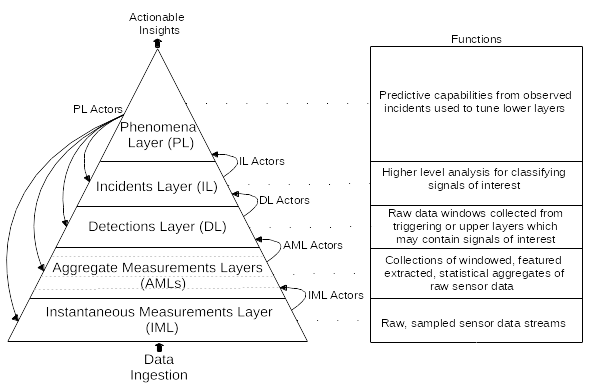
\includegraphics[width=4in]{images/mauka/mauka-data-model.png}
\caption{Mauka data model hierarchy}
\label{fig:mauka-data-model}
\end{figure}

\begin{tcolorbox}[colback=red!5!white,colframe=red!75!black,title=ANTHONY]
Please review the following paragraphs for accuracy and quality.
\end{tcolorbox}

In essence, the raw data sent to the cloud from OPQ Boxes is initially stored in the Instantaneous Measurements Layer (IML). IML Actors process this data to determine if additional data from OPQ Boxes are warranted, and request this data if necessary. This data, along with the instantaneous data, is then stored at the Aggregate Measurement Layer (AML).  All data from the IML layer is discarded after one hour if it is not found to be interesting and thus promoted to the AML level. Once at the AML Layer, AML actors process the augmented data sets to determine if they constitute an actual power quality anomaly, and if multiple OPQ Boxes appear to be implicated in the anomaly. If so, all of the associated AML data is promoted to the Incident Layer (IL).  AML data must be promoted within one day or else it is discarded.  Finally, IL Actors are responsible for looking for ways to make Incidents actionable, and if successful, will promote the IL data to the Phenomena Layer (PL). For example, if the same boxes are generating the same Incidents on a periodic basis, then these Incidents could be promoted to a Phenomena that can predict when the next occurrence of this Incident might occur.

While IML, AML, DL, and IL Actors all promote data upward, the Phenomena Actor actually works in the opposite direction, using its knowledge to configure lower levels. For example, if a periodic Phenomena has been created, then a PL Actor might alter the behavior at the AML, gathering more raw data from Boxes around the time of the next predicted Incident.


\subsection{OPQ Mauka Actors}

The current capabilities of OPQ Mauka can be summarized in terms of its Actors, which are implemented as plugins.

{\em BasePlugin.} All Actor plugins derive from the BasePlugin, which provides primitives for running plugins as separate processes, serialization and deserialization of type safe messages, communication over ZeroMQ, metrics collection, MongoDB communication, debugging, and plugin health.

{\em MakaiEventPlugin.} The MakaiEventPlugin Actor is responsible for reading Events newly created by OPQ Makai into OPQ Mauka. It performs feature extraction on the raw Event data streams and forwards those features (or the raw data) to subscribing plugins. This allows OPQ Mauka to perform feature extraction once, and reuse those features in multiple plugins.

{\em FrequencyVariationPlugin.} The FrequencyVariationPlugin is used to classify generic frequency sags, swells, and interruptions as defined by the IEEE 1159 standard. Both duration and deviation from nominal are used to perform these classifications. Duration classifications include frequency deviations that last for less than 50 ns, between 50 ns to 1 ms, and 1 ms to 50 ms. Classifications for deviations from nominal are performed for values that are up to 40\% deviation from nominal. The plugin is able to classify frequency swells, frequency interruptions, and frequency sags. When a new frequency variation is detected, a frequency Incident is created.


{\em IEEE1159VoltagePlugin.} The IEEE1159VoltagePlugin is used to classify voltage Incidents in accordance with the IEEE 1159 standard[29]. In general, this standard classifies voltage disturbances by duration and by magnitude. Voltage durations are classified from 0.5 to 30 cycles, 30 cycles to 3 seconds, 3 seconds to a minute, and greater than 1 minute. Voltage deviations are classified in both the sag and swell directions as a percentage from nominal. Sags are generally classified between 10\% and 90\% of nominal while swells are generally classified from 110\% to 180\% of nominal. This plugin is capable of classifying voltage sags, swells, and interruptions as defined by the standard. The plugin works by identifying sags, swells, and interruptions and determining the duration of those Events. If the duration or delta is large enough, a voltage Incident is created.

{\em BoxOptimizationPlugin.} The BoxOptimizationPlugin is responsible for sending and receiving typed messages to and from OPQ Boxes from OPQ Mauka. This plugin is capable of requesting the state of each OPQ Box (e.g. uptime, Measurement rate, security keys, etc). This plugin is also capable of adjusting the state of individual OPQ Boxes by changing things such as the Measurement and Trend rate or the sampling rate that the Box is sampling at.

{\em FuturePhenomenaPlugin.} The FuturePhenomenaPlugin is responsible for creating Future or Predictive Phenomena. These Phenomena are used to predict Events and Incidents that may occur in the future. This plugin does not subscribe to any messages, but instead utilizes timers to perform its work. By default, this plugin runs every 10 minutes.

When the plugin runs, it loads any active Periodic Phenomena found in the database. If Periodic Phenomena are found, this plugin extrapolates possible Events and Incidents by first examining the timestamps of previous periods and then extrapolating into the future using the mean period and the standard deviation. For each timestamp in the periodic phenomena, the mean period is added. If the resulting timestamp is in the future, a Future Phenomena is created using the time range of the future timestamp plus or minus the standard deviation of the Periodic Phenomena.

When a Future Phenomena is created, timers are started in a separate thread signifying the start and end timestamps of the Future Phenomena. When the first timer runs, messages are sent to the BoxOptimizationPlugin and the ThresholdOptimizationPlugin instructing Event thresholds to be set lower and Box Measurement rates to be set higher. This increases the chance of seeing an Event over the predicted time window. When the second timer runs, these values are reset to their default values. Thus, the plugin increases fidelity and decreases thresholds over the period of a Future Phenomena.


{\em ITICPlugin.} The ITICPlugin analyzes Vrms to determine where it falls within the ITIC curve \cite{thallam_power_2000}. The ITIC curve is a power acceptability curve that plots time on the x-axis and Vrms on the y-axis.  The purpose of the curve is to provide a tolerance envelope for single-phase 120V equipment. The curve defines three regions. The first region is "No Interruption" and generally includes all voltages with very short sustained durations. All events within this region have no noticeable effect on power equipment. The second region, the "No Damage Region", occurs during voltage sags for extended periods of time. Power Events in this region may cause equipment interruptions, but it will not damage the equipment. The final region, the "Prohibited" region, is caused by sustained voltage swells and may cause damage to power equipment. This plugin determines if an event falls within the "No Damage" or "Prohibited" regions and if so, creates an Incident to record this.

{\em SemiF47Plugin.} The SemiF47 plugin is another plugin like the IticPlugin that plots voltage and duration against a power acceptability curve. In this case, the standard used is the SemiF47 standard \cite{djokic_sensitivity_2005}. Rather than using a point-in-polygon approach, this plugin reads the VRMS features sequentially and uses a state machine to keep track of the current classification. This plugin only classifies values as a "violation" or as "nominal".

{\em TransientPlugin.} The "TransientPlugin" is responsible for classifying frequency transients in power waveforms. The plugin subscribes to messages from the "RawVoltage" topic which contains a calibrated power waveform payload. The TransientPlugin is capable of classifying impulsive, arcing, oscillatory, and periodic notching transients. A decision tree is utilized to select the most likely transient type and then further analysis is used to perform the actual classification of transients. Dickens et al \cite{dickens_transient_2019} provides more details on the transient classification system.

{\em PeriodicityPlugin.} The "Periodicity Plugin" is responsible for detecting periodic signals in power data. This plugin does not subscribe to any messages, but instead runs off of a configurable timer. The plugin is set to run by default once an hour and every hour it scrapes the last 24 hours worth of data and attempts to find periods in the Measurements over that duration.

For each feature in the Measurement and Trend data (e.g. frequency, voltage, and THD), the Periodicity plugin first removes the DC offset from the data by subtracting the mean. Next, the plugin filters the signal using a 4th order high-pass filter to filter out noise. The plugin then performs autocorrelation on the signal followed by finding the peaks of the autocorrelation. The mean distance between the peaks of the autocorrelation provides the period of the signal.

The plugin only classifies data as periodic if at least 3 peaks were found and the standard deviation of the period is less than 600 seconds (10 minutes). Once a positive identification has been made, peak detection is performed on the original signal. Once the plugin has the timestamps and deviations from nominal of the periodic signal of interest, the plugin can group Measurements, Trends, Events, and Incidents that were created during the periodic signals together as part of the Periodic Phenomena.



